\chapter{Results} \label{chap:results}
\begin{toReview}
\section{Architecture}
	As mentioned in the previous chapters, the image analysis system requires the comparison of an unknown work with known ones.

	\noindent The image is pre-processed to remove non-handwriting artefacts, resulting in a greyscale image where the author's handwriting appears as dark tones on a white background. In addition, the thickness of the author's strokes may need to be adjusted relative to the printed characters, and the resolution (expressed in \gls{ppi}) must match the dataset specifications.

	\noindent The pre-processed image is then synthesised: a program extracts tiles of a certain size, according to the requirements of the dataset. The image is then compared with each image in the dataset (or with the most representative images for each author).

	\noindent This chapter provides an analysis of each step outlined in this thesis, evaluating the impact of each component on the images studied. It also analyses and justifies the decisions and parameters chosen during the design phase.

	\bigskip
	\noindent Each image with a known author is fully compared to all other known images. Since the comparison value is symmetric, only half of all possible comparisons need to be evaluated. For $n$ images, imagine filling a square $n\times n$ table with real values. Assuming a comparison value of $0$ between identical images, the total number of comparisons required is $\frac{n^2-n}{2}$.

	\noindent For this reason, the algorithm computes only half of the comparisons for each row, as shown in \cref{fig:distance_computation}. Specifically
	\begin{itemize}
		\item If $n$ is odd, each row performs $\frac{n-1}{2}$ comparisons (with the remaining values derived by symmetry).
		\item If $n$ is even, $\frac{n}2$ comparisons are performed for even-indexed rows (where the first row has index $0$), while $\frac{n}2-1$ comparisons are performed for odd-indexed rows.
	\end{itemize}
	\noindent This method provides a more uniform analysis for large datasets, especially when combined with row and column shuffling.

	\begin{figure}[H]
		\centering
		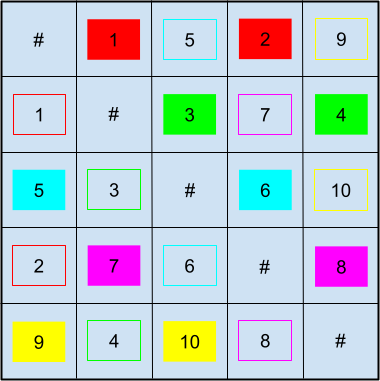
\includegraphics[width=0.7\linewidth]{Figures/analysis_sort.png}
		\caption[Visit all pairs combinations of a list]{The algorithm calculates half of all components for each row. In the figure, the algorithm follows the order of the numbers, taking cells alternately so that the bottom diagonal is not directly computed and the top diagonal is directly computed. For example, in the row $3^\text{-th}$, the algorithm directly computes the first column (number $5$ in cyan) and the penultimate column (number $6$ in cyan), while the second column is already computed (number $3$ in green square) and the last column is not yet computed.}
		\label{fig:distance_computation}
	\end{figure}

	\subsection{Challenges} The implementation of the code presented significant challenges, as many of the required frameworks did not exist, and computational and time constraints posed additional hurdles. This necessitated the development of highly efficient and sophisticated code to optimise computational performance.

	\noindent The project is heavily based on \gls{Python} and \gls{CUDA}. Specialised debugging, logging and testing software was used extensively to ensure that the software worked correctly. Automated documentation tools and version control systems were used to manage and track code development. In addition, a robust error handling and session management system was implemented, which included backup mechanisms (called "checkpoints") to prevent the loss of valuable data. Temporary files were also used to extend storage capacity beyond the limits of primary storage.

	\noindent Due to its complexity and length (a total of almost $4000$ lines), the code cannot be fully included in this document. However, it is available in the \gls{github} repository:\\ \url{https://github.com/StefanoMagriniAlunno/MMATH_thesis}.

	\bigskip\noindent The code uses wrapping, which allows a \gls{Python} script to interface with pre-compiled \gls{cxx} code. This approach allows the \gls{Python} script to handle high-level tasks such as preparing input files and reports, retrieving hardware specifications, and configuring computing sessions. When intensive computations are required, the \gls{Python} script calls precompiled \gls{cxx} libraries, ensuring that the \gls{cxx} code remains streamlined and more readable.

	\noindent For example, when initiating a comparison between works, the main \gls{Python} script prepares the operating system environment, validates the parameters used, and handles any existing checkpoints. It then passes all necessary input to the wrapper (written in \gls{cxx}), which validates syntax errors and translates Python types into \gls{cxx}-compatible types. The wrapper then calls a starter function which initialises logging mechanisms and reads input files, effectively setting up main memory. The \gls{cxx} program then calls the \gls{cuda} program, which reads the GPU specifications (using dedicated libraries) and configures a computation plan to maximise performance and ensure robustness. Finally, the \gls{gpu} receives kernel instructions that it compiles at runtime to perform the computations. Given the limited memory of \gls{gpu}s, data is transferred in chunks, with main memory acting as a buffer.

	\noindent The results computed by the GPU are returned to the calling \gls{cxx} function, which stores them appropriately and returns control to the calling \gls{Python} script. In case of errors, all relevant information is documented and passed back to the caller for appropriate handling.

	\noindent These strategies for developing high-performance code are common in scientific computing libraries, which often have a main calling function with hidden compiled functions. An example is CuPy, a \gls{Python} library that requires compilation as part of its installation process.

	\section{pre-Processing}
	pre-Processing is a critical stage in the comparison of unknown works with the dataset. Its primary objective is to ensure that the quality specifications of the images meet certain standards. These specifications are often subjective, and it is not guaranteed that the same algorithm will be applied to each image. The ultimate goal is to remove clearly contaminating data, standardise the image quality and prepare it for analysis by the software. Essentially, pre-processing transforms the real data into an ideal format that is theoretically acceptable to the software.

	\noindent As previously illustrated in \cref{alg:CleaningFFT}, the pre-processing applied to the collected data primarily involves compression using the \gls{fft}. This section presents a step-by-step analysis of the results produced by the algorithm.
    \paragraph{FFT}
    The first step of the pre-processing algorithm is to apply \gls{fft} to the normalised image, where pixel values have a mean of $0$ and a variance of $1$. As noted in the summary images, the grid patterns in the background of the notebook pages are recurring features that are not typical of writing. These recurring patterns are more apparent when Fourier transforms are used.

    \noindent In \cref{fig:fft_application} the grid pattern is visible as high-intensity frequencies almost aligned along the sides.
\newpage
    \begin{figure}[H]
    	\centering \includegraphics[width=1.0\linewidth]{Figures/fft_application.png}\caption[FFT application in pre-processing]{Significant frequencies along the edges of the second image reveal the grid pattern.}\label{fig:fft_application}
    \end{figure}

	\noindent The algorithm removes the $p$ percentile of the frequencies with the highest amplitude and reconstructs the original image using the remaining frequencies whose amplitudes are preserved. In \cref{fig:fft_percentile} different reconstructions using different percentiles are shown, with pixel intensities normalised between $0$ and $1$. The results suggest that $p=0.1\%$ is a reasonable starting point for analysis.

	\begin{figure}[H]
		\centering \includegraphics[width=1.0\linewidth]{Figures/fft_percentile.png}\caption[Comparing different percentiles in FFT]{A percentile between $0.1\%$ and $0.05\%$ strikes a good balance by removing the grid patterns while leaving the handwriting intact.}
		\label{fig:fft_percentile}
	\end{figure}

	\noindent While normalisation makes these images visually comparable, it masks the fact that the pixels in the reconstructed images tend to have very similar intensities. To overcome this, the algorithm identifies pixels that were certainly part of the white background or handwriting in the original image. Specifically
	\begin{itemize}
		\item Pixels with intensity below $0.2$ are considered part of the handwriting.
		\item Pixels with intensity above $0.8$ are considered part of the white background.
	\end{itemize}
	\noindent Using this analysis, the algorithm calculates how many pixels belong to the handwriting and how many belong to the background. \cref{fig:fft_diagrams} illustrates this analysis.

	\begin{figure}[H]
		\centering 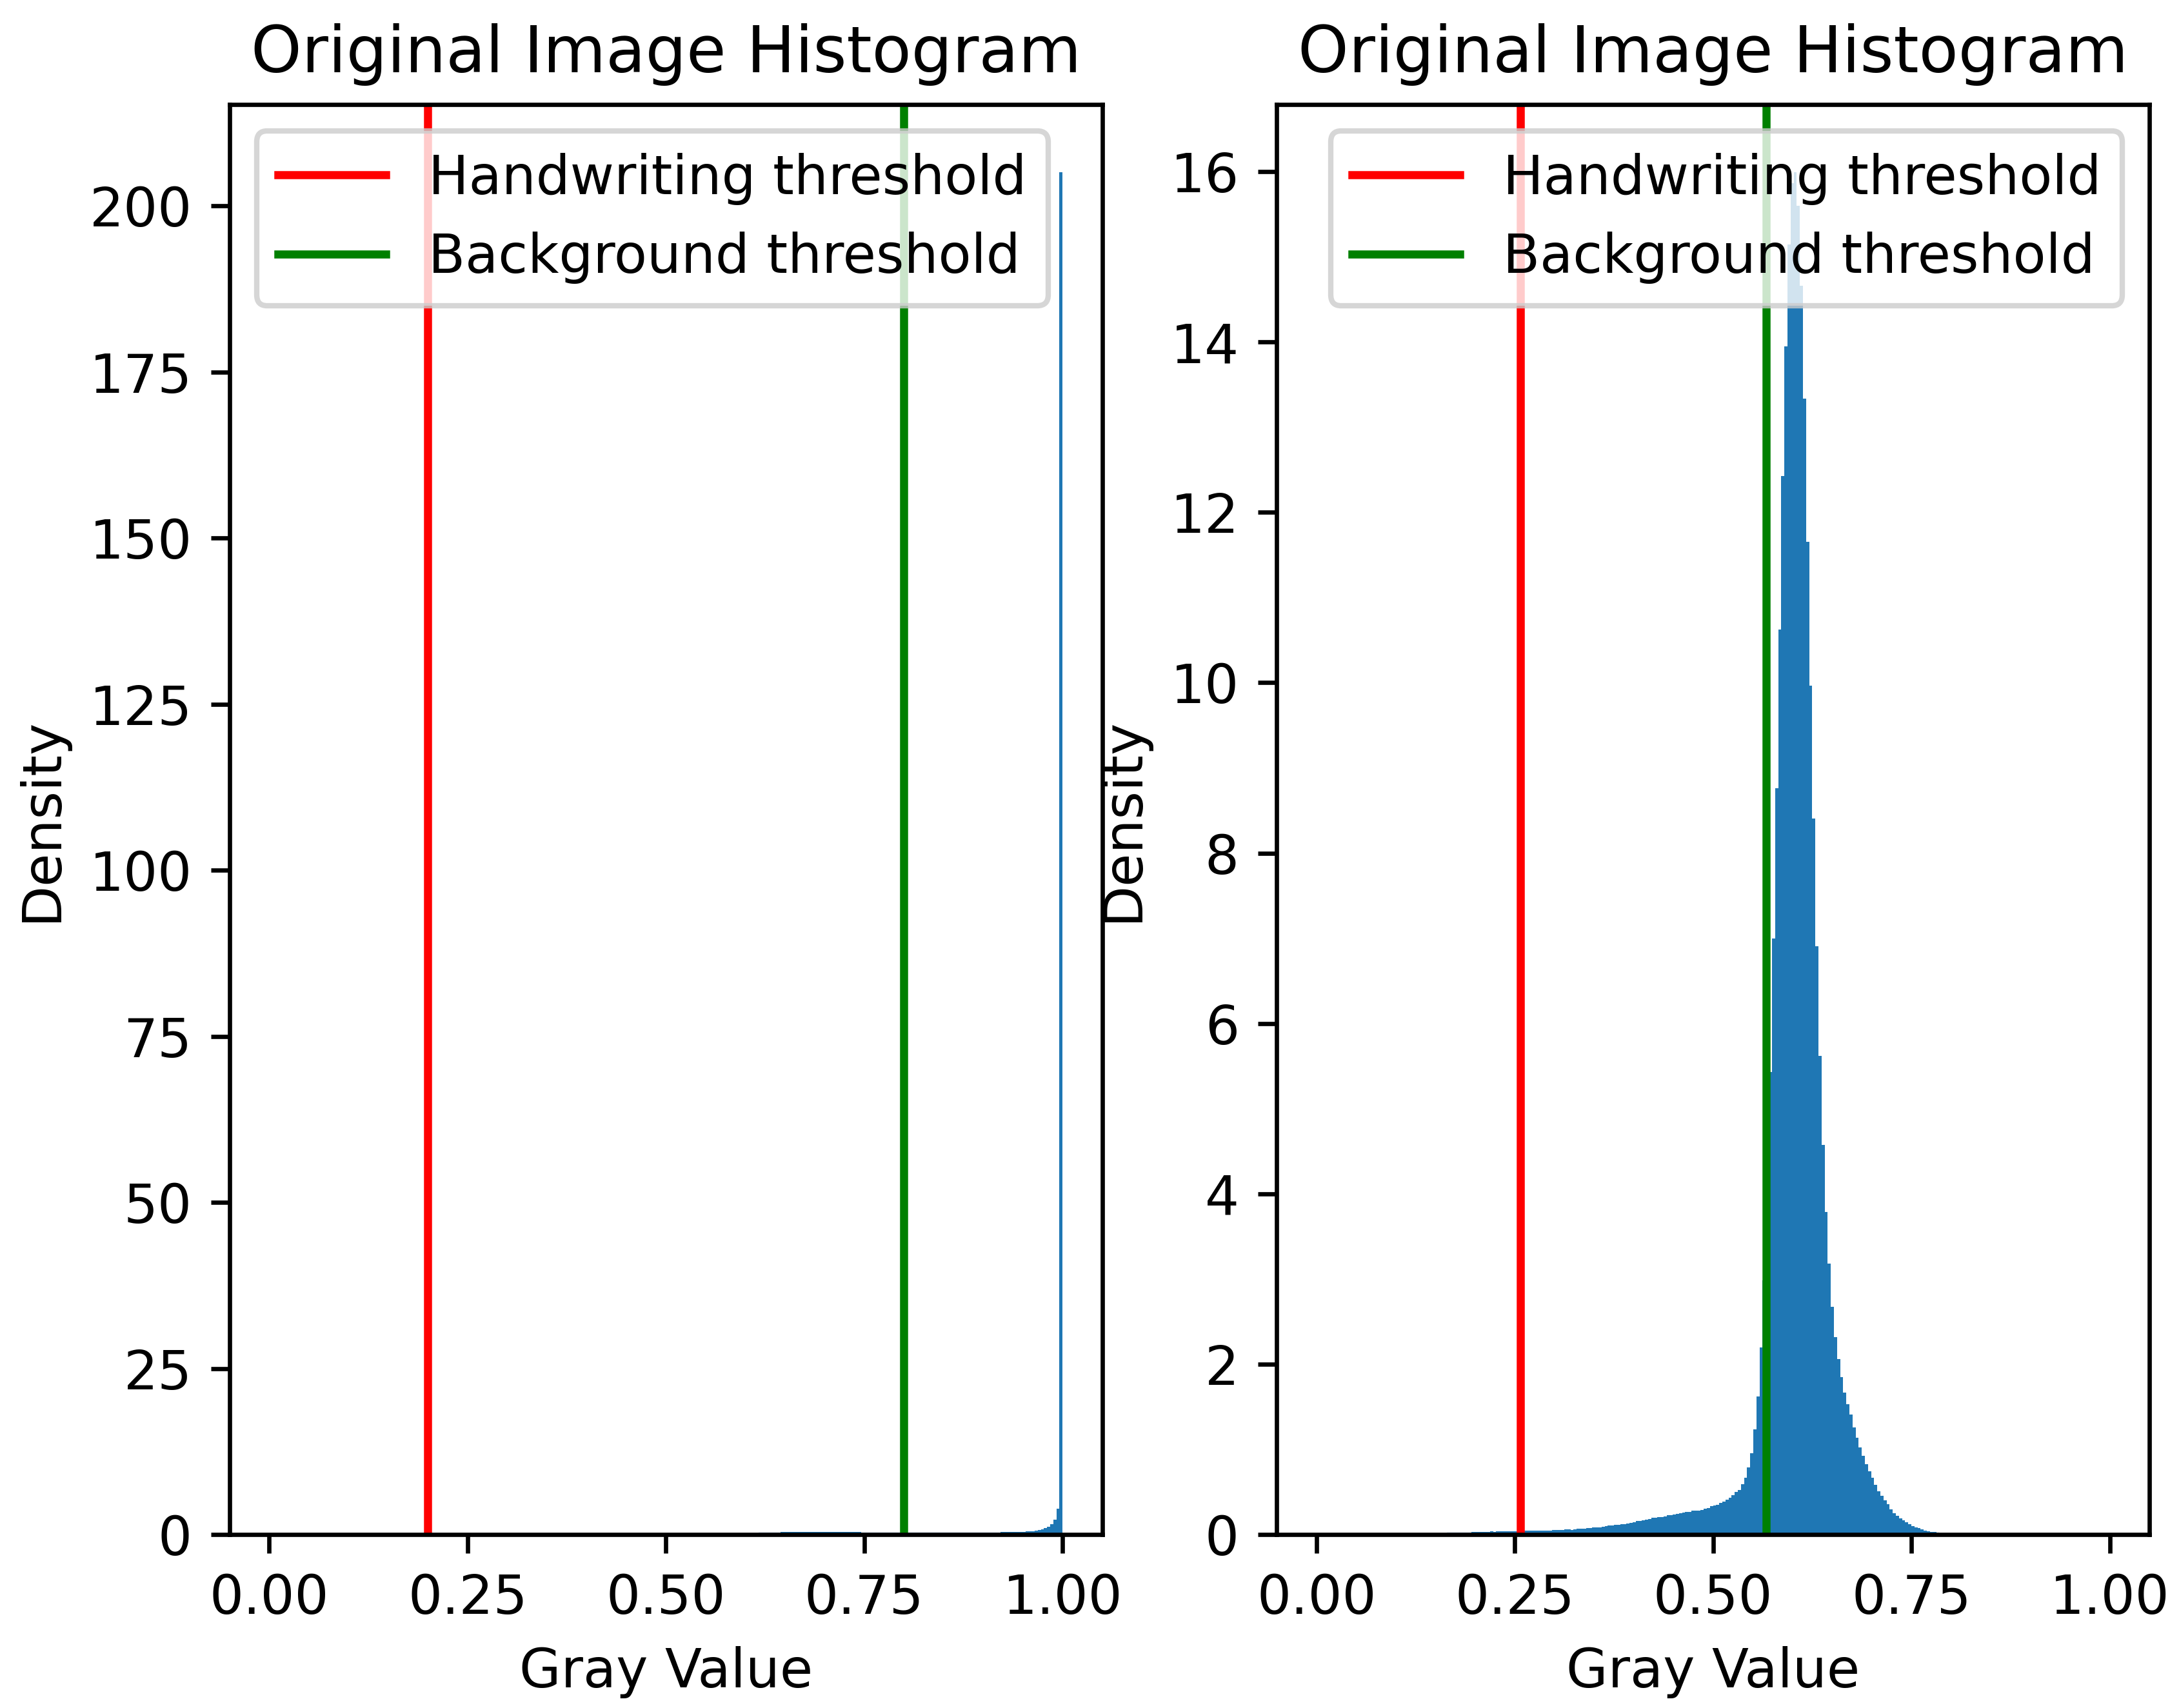
\includegraphics[width=0.8\linewidth]{Figures/fft_diagrams.png} \caption[Density changes after FFT compression]{In the original image, most pixels are white, while the reconstructed image contains more mid-grey pixels. To preserve the original distribution, thresholds are computed based on the original image: pixels above $0.8$ (green line) are assumed to be background, while pixels below $0.2$ (red line) are assumed to be handwriting. These thresholds are used to define two new boundaries in the reconstructed image.} \label{fig:fft_diagrams}
	\end{figure}

	\noindent The algorithm identifies two thresholds in the reconstructed image:
	\begin{itemize}
		\item $\texttt{h}_\texttt{up}$: Above this intensity, the number of pixels matches (or slightly underestimates) the number of background pixels in the original image.
		\item $\texttt{h}_\texttt{down}$: Below this intensity, the number of pixels matches (or slightly underestimates) the number of handwriting pixels in the original image.
	\end{itemize}
	\noindent A linear transformation is applied to the pixel intensities in the reconstructed image to scale these thresholds to $1$ and $0$ respectively:
	\[
	\texttt{gray}_\texttt{new} = \frac{\texttt{gray}_\texttt{old} - \texttt{h}_\texttt{down}}{\texttt{h}_\texttt{up} - \texttt{h}_\texttt{down}}
	\]
	\noindent Pixel intensities outside the range $[0,1]$ are clamped to $0$ or $1$ using the \texttt{clamp} function.
	\[
		\texttt{clamp}\left(\texttt{gray}_\texttt{new}\right) = \begin{cases}
			0 & \textnormal{if} \quad \texttt{gray}_\texttt{new} < 0 \\
			1 & \textnormal{if} \quad \texttt{gray}_\texttt{new} > 1 \\
			\texttt{gray}_\texttt{new} & \textnormal{otherwise}
		\end{cases}
	\]

	\noindent The \cref{fig:fft_results} shows the results of this process for $p=0.1\%$ and $p=0.05\%$ on two samples. While the results appear visually similar, using $p=0.05\%$ preserves the handwriting better, but at the cost of retaining some lattice artefacts. It is hoped that this residual noise will be captured by the \gls{fcm} clustering.

	\begin{figure}[H]
		\centering 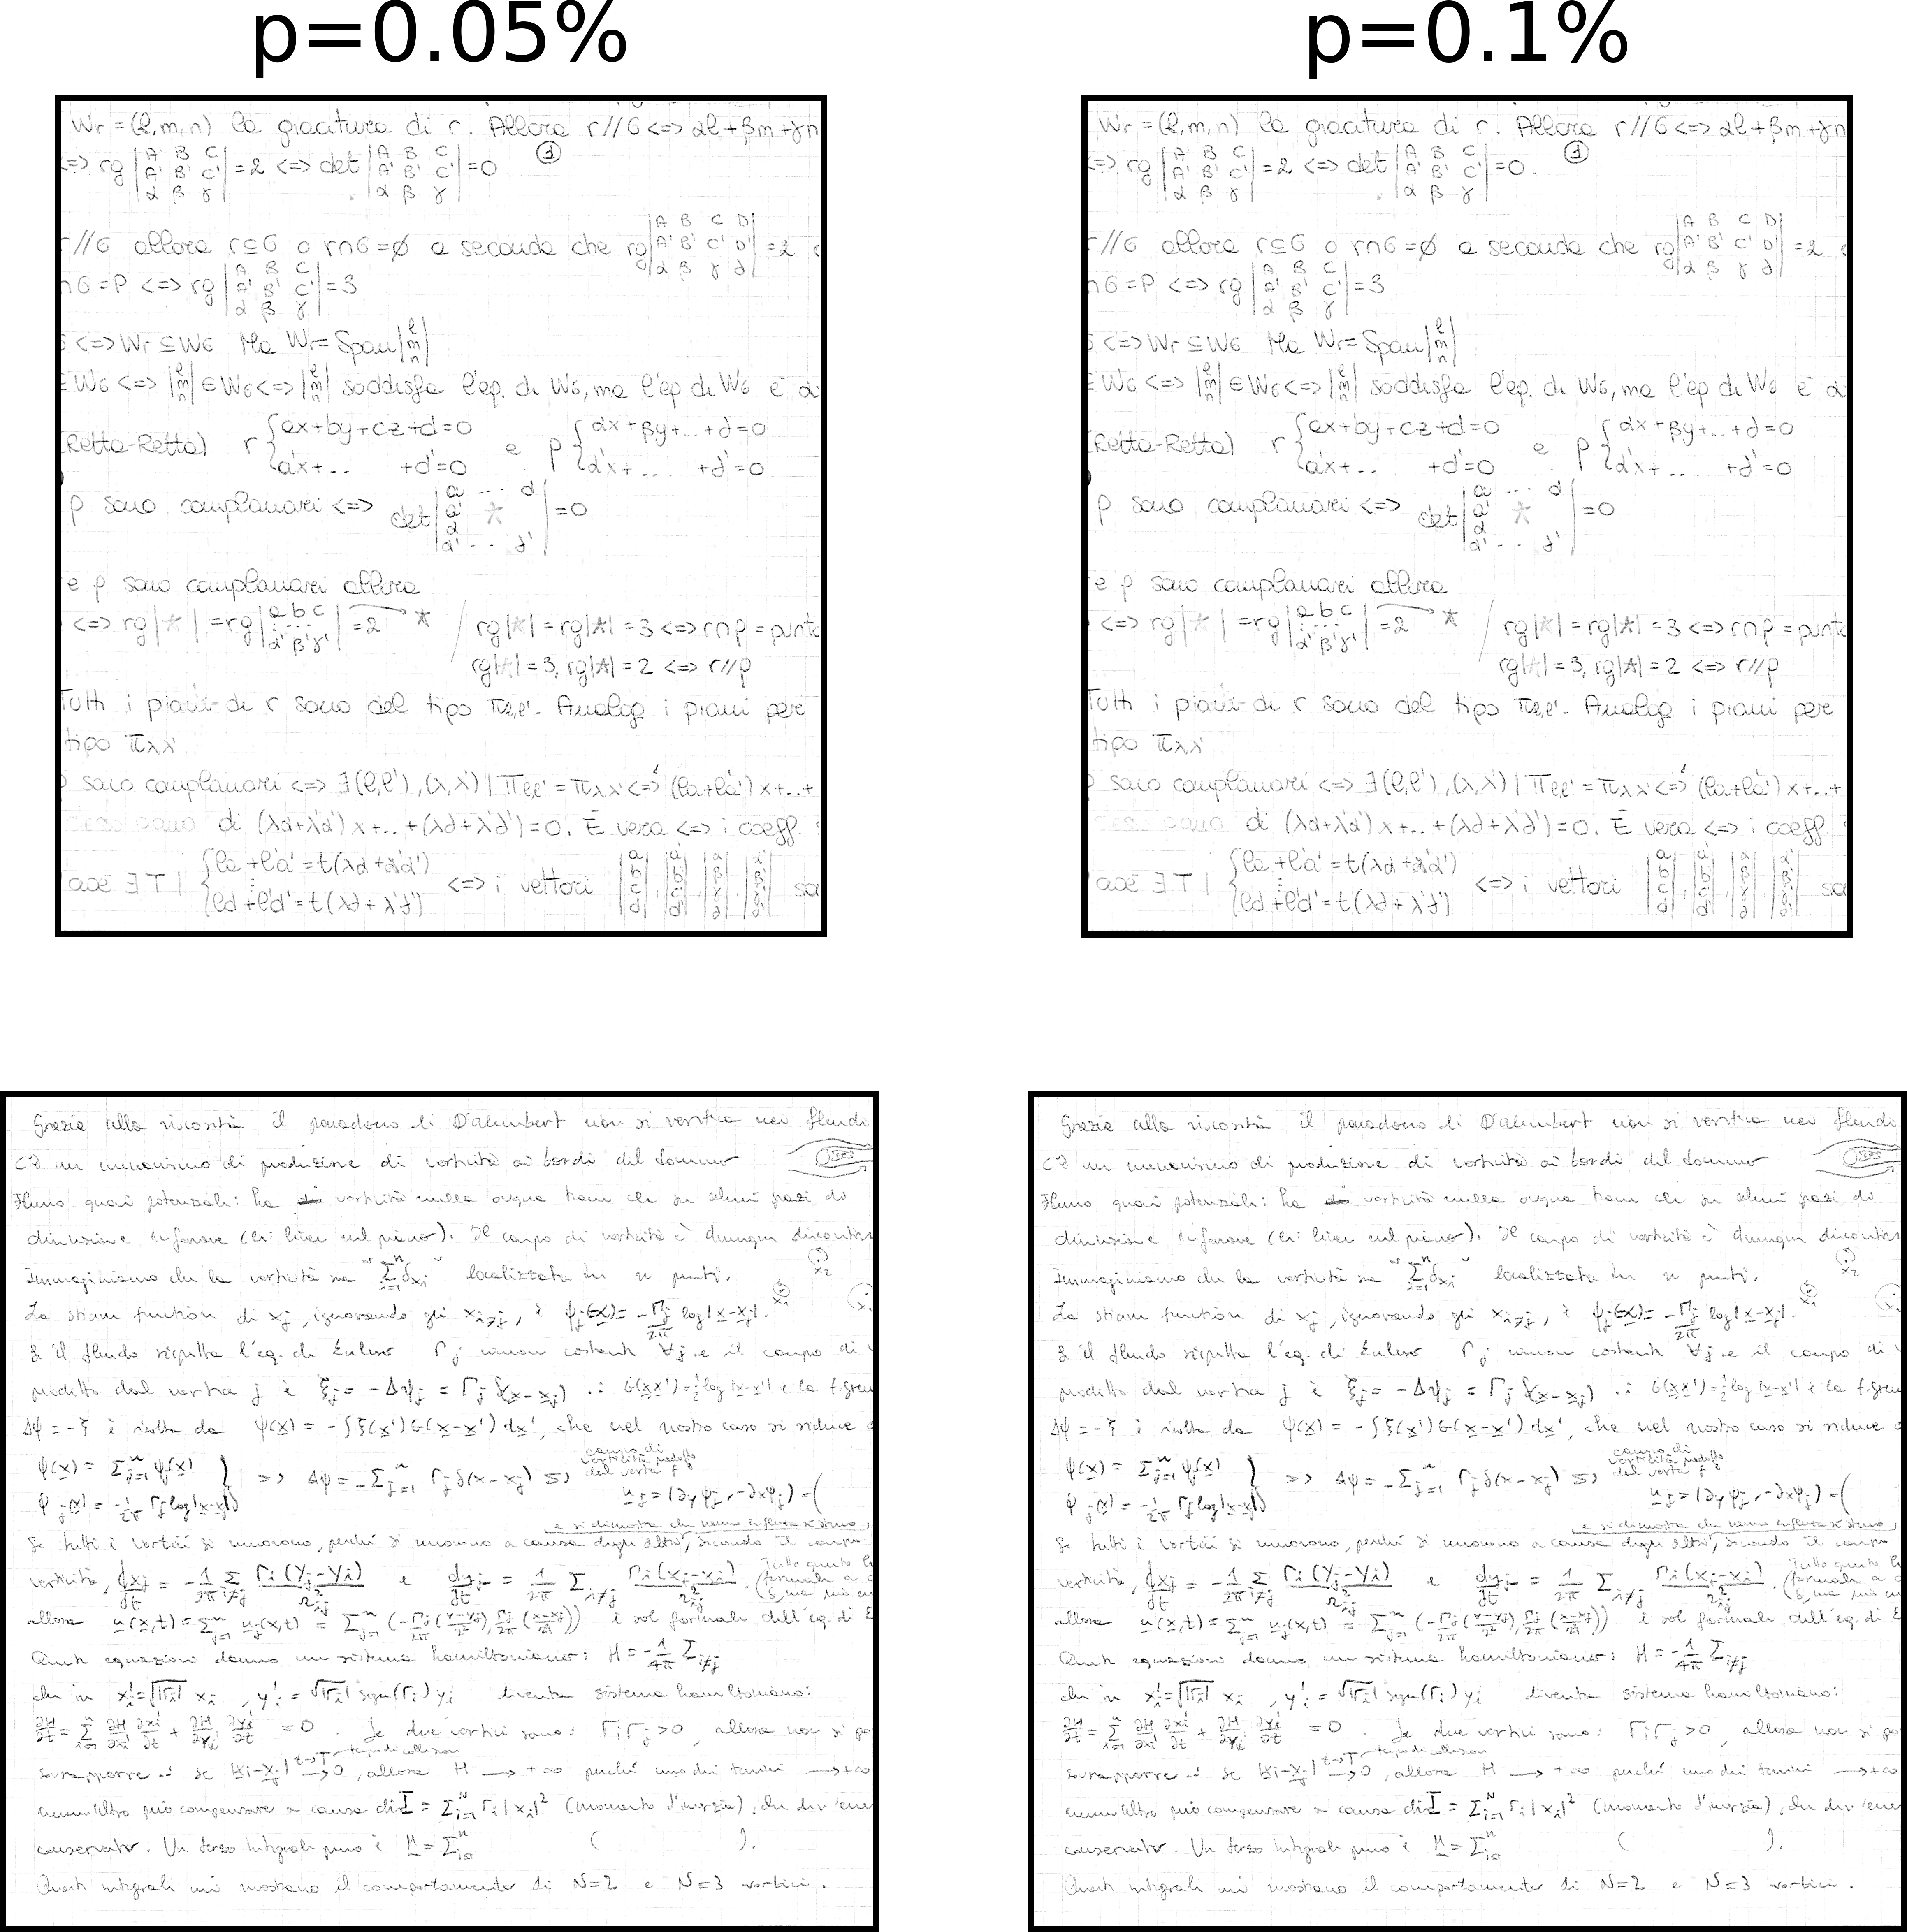
\includegraphics[width=1.0\linewidth]{Figures/fft_results.png} \caption[Results of the FFT cleaning process]{Two pre-processed images with different percentiles are shown. The first column corresponds to $p=0.05\%$ and the second column corresponds to $p=0.1\%$. Each row represents one work from the dataset.} \label{fig:fft_results}
	\end{figure}

    \section{Synthesis} Once the images have been pre-processed and adapted to the data set according to "human" parameters, the synthesis phase begins. This step ensures that the works are redefined in an objectively consistent manner. Specifically, the works are transformed into an (ordered or unordered) list of square tiles with uniform sizes.

    \noindent As mentioned above, the \gls{Python} script manages the operating system and efficiently retrieves input and hardware parameters for lower level pre-compiled programs. In this case, the \texttt{synthesis.py} script sets up the necessary directories to allow a \gls{cxx} program to store the generated syntheses. This process is achieved using a simple code structure as shown below:

\begin{lstlisting}[style=code, language=C, rulecolor=\color{blue}]
/** @brief In this code we use OpenMP API to realize an array with all tiles.
 *
 *  @param[in] byte_board : the array with all pixels
 *  @param[out] cells : the array with all tiles of the image
 *  @param n_threads : the number of used threads in the first loop
 *  @param height : the height of the image
 *  @param width : the width of the image
 *  @param n_tiles : the size of tiles
 *
 *  @details This code uses a bijective map from tiles and "short"image, i.e. an image with shape width_short, height_short. Each tiles will be assigned to its first pixel (up/sx).
 *  "omp parallel for" is a directive of OpenMP that executes a for cycle using more indipendent threads. In this case the schedule is "static" i.e. each thread knows in advance all its loops.
 */
unsigned width_short = width - n_tiles + 1,
         height_short = height - n_tiles + 1;
#pragma omp parallel for schedule(static) num_threads(n_threads)
for (unsigned row = 0; row < height_short; ++row)
for (unsigned col = 0; col < width_short; ++col)
  for (unsigned i = 0; i < n_tiles; ++i)
  for (unsigned j = 0; j < n_tiles; ++j) {
    long unsigned index_out = ((row * width_short + col) * n_tiles + i) * n_tiles + j; // [row-i, col-j, i,j]
    long unsigned index_in = (row + i) * width + col + j;
    cells[index_out] = byte_board[index_in];
    }\end{lstlisting}

    \noindent Using multiple \gls{thread}s to execute a loop significantly improves performance, achieving a multiplicative speedup. In addition, write access to \texttt{cells} for different \texttt{row}s does not raise concurrency issues, such as multiple \gls{thread}s attempting to write to the same memory location. In this case, the nominal execution time of the loop does not depend on the choice of row. For this reason, a static scheduling strategy greatly reduces the overhead associated with managing the set of generated threads.

    \noindent Multi-threading techniques are primarily used to optimise the execution time of small, parallelizable tasks. It is unusual to apply such techniques at a high level, such as analysing two images simultaneously. While starting multiple high-level processes can reduce overall startup times, it also increases memory requirements. The suitability of this method depends largely on the specific problem being solved.

    \noindent Since each image is transformed into a set of tiles, it is obvious that this can significantly increase memory usage. The number of elements in the \texttt{cells} array is given by:\\ $(w-n+1)(h-n+1)n^2$, where $w$ and $h$ are the dimensions of the original image and $n$ is the size of the tiles. As a result, managing multiple high-level threads becomes challenging due to the significant memory requirements.
	\newpage
    \subsection{A Simple Analysis} Since syntheses are represented as sets of high-dimensional points, visualising them can be challenging. To address this, we propose a "coarse" visualisation technique that reduces the dimensionality from $\mathbb{R}^{16}$ (for $4\times4$ tiles) to $\mathbb{R}^6$. This reduction is achieved using \gls{pca}, and only a subsample of $\num{5000}$ tiles is visualised. It is important to note that this approach introduces a significant loss of both dimensionality and data quantity, so the proposed plots are purely illustrative.

    \noindent As shown in \cref{fig:synth_glbvisual}, there is a region where the tiles are densely clustered. The most reasonable hypothesis is that the background of the images produces many bright tiles that form a dense cluster. To confirm this hypothesis, these points are highlighted and linked to their original tiles.

    \begin{figure}[H] \centering 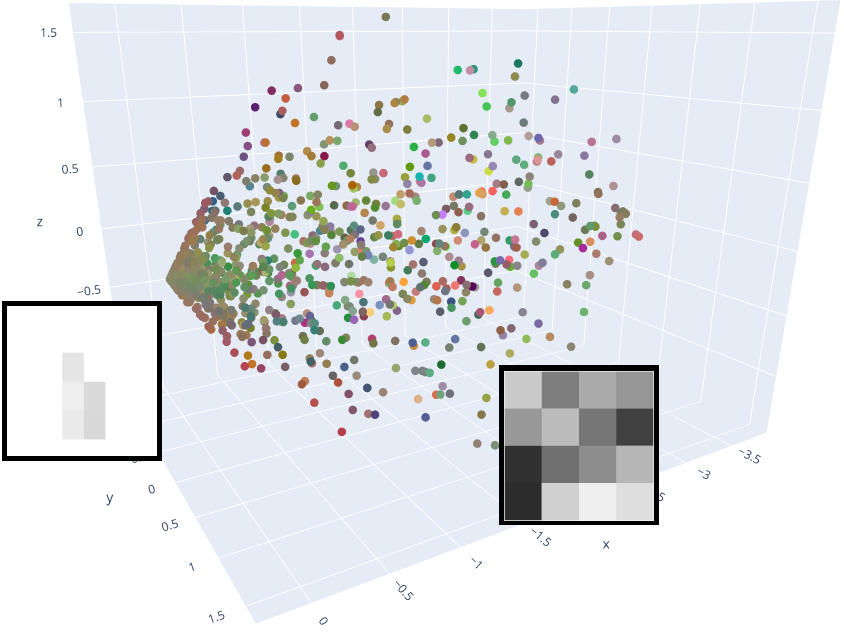
\includegraphics[width=0.8\linewidth]{Figures/synth_glbvisual.png}
    	\caption[Global visualisation of a synthesis using PCA]{The figure shows a scatterplot of a sample of tiles extracted from an image. Six dimensions are represented using colours. As can be seen, the background tiles are mostly concentrated around $0$, while the handwriting tiles are more scattered.}
    	\label{fig:synth_glbvisual}
    \end{figure}
	\newpage
    \section{Comparison} The comparison between distributions defines the dissimilarity between works. Given the computational cost of this process, it is important to analyse the trade-off between the quality of the result and the time required, as well as the parameters chosen. Specifically, the following strategies are considered:
    \begin{itemize}
    	\item Reducing the number of iterations used to calculate the centroid in \gls{fcm}.
    	\item Reduce the number of centroids in \gls{fcm}.
    	\item Reduce dimensionality using \gls{pca} before running \gls{fcm}.
    	\item Reducing the number of data points before running \gls{fcm}.
    \end{itemize}

	\subsection{Implementation} The implementation of the comparison algorithm is long and complex; only a general framework is presented here. Specifically, we focus on how the data is managed by the \gls{gpu}, taking into account its physical limitations.

	\noindent Examining the update formulas reveals the possibility of performing updates using batches. Due to the memory limitations of the \gls{gpu}, it is not possible to compute a complete update in one step. Instead, partial computations must be accumulated in smaller batches of data.

	\noindent The theoretical update formulae are as follows
	\begin{align*}
		c_{j}^\text{new} &= \frac{\sum_{i=1}^N u_{ij}^2w_ix_i}{\sum_{i=1}^N u_{ij}^2w_i}, \\
		u_{ij} &= \frac{1}{\sum_k\frac{d_{ij}^2}{d_{ik}^2}}, \\
		d_{ij} &= \left\|x_i - c_{j}\right\|
	\end{align*}

	\noindent A single iteration step can be further subdivided into steps across batches, indexed here by $B$:
	\begin{equation*}
		C_{j}^\text{new} = \frac{\sum_{B}\sum_{i\in B} u_{ij}^2w_ix_i}{\sum_{B}\sum_{i\in B} u_{ij}^2w_i}
	\end{equation*}

	\noindent Consequently, the communication between the host (the programme flow executed by the \gls{cpu}) and the device (the programme flow executed by the \gls{gpu}) can be simplified as follows:
	\newpage
	\begin{algorithm}[H]
		\caption{Host/Device communication\\
			\textsc{INPUT}\\
			$\bullet$ $\mathcal{X}$: set of data $x_1,\ldots,x_N\in\mathbb{R}^K$ and weights $w_1,\ldots,w_N$\\
			$\bullet$ $\mathcal{C}$: centroids $c_1,\cdots,c_M$\\
			$\bullet$ stop: stop criteria of the clustering (a positive value)
		}
		\begin{algorithmic}[1]
			\Function{FCMwrapper}{$\mathcal{C}$, $\mathcal{X}$, $\text{stop}$}
				\State $v^\text{num} \gets $ array with $M$ vectors in $\mathbb{R}^K$ into the Device
				\State $v^\text{den} \gets $ array with $M$ real values into the Device
				\State $\mathcal{C}'$ a copy of centroids $\mathcal{C}$ into the Device
				\State $s \gets \infty$
				\State $L \gets \infty$
				\While{$s > \text{stop}$}
					\State Compute batch size
					\State $v^\text{num}\gets \vec{0}$
					\State $v^\text{den}\gets \vec{0}$
					\State $L_\text{new} \gets 0$ \Comment Current value of loss function, see \cref{def:fuzzyloss}
					\For{each $B$ batch}
						\State move $B$ into the Device
						\State Call the data points of $B$ as $x$
						\State Call the weights of $B$ as $w$
						\State Compute $U^2, D^2$ between $B$ and $\mathcal{C}'$ \Comment calling \cref{alg:MembershipUpdateSafe}
						\State $L_\text{batch} \gets \sum_{i,j}u_{ij}^2d_{ij}^2$
						\State $v^\text{num}_\text{batch} \gets \sum_{i} u_{ij}^2w_ix_i\quad\forall j$
						\State $v^\text{den}_\text{batch} \gets \sum_{i} u_{ij}^2w_i\quad\forall j$
						\State $v^\text{num} \gets v^\text{num} + v^\text{num}_\text{batch}$
						\State $v^\text{den} \gets v^\text{den} + v^\text{den}_\text{batch}$
						\State $L_\text{new} \gets L_\text{new} + L_\text{batch}$
					\EndFor
					\State $C'_j \gets \frac{v^\text{num}_j}{ v^\text{den}_j} \quad \forall j$
					\State $s \gets L - L_\text{new}$
					\State $L \gets L_\text{new}$
				\EndWhile
				\State move $\mathcal{C}'$ into the Host
				\State \Return $\mathcal{C}'$
			\EndFunction
			\label{alg:FCMwrapper}
		\end{algorithmic}
	\end{algorithm}

	\noindent The computation of the $U^2$ matrix and $L_\text{batch}$ is performed simultaneously, without the need to store $D^2$. This computation is performed by a \gls{cuda} kernel whose pseudocode is presented in \cref{alg:MembershipUpdateSafe}, with implementation details in \cref{appendix:fcm_kernel}. The computational cost for each batch is $O(\log KM)$.

	\bigskip\noindent Hardware limitations may limit the size of the batch, both due to memory constraints and parallelism limits.

	\noindent The use of \gls{gpu} greatly improves performance. This has already been discussed in general terms in \cref{chap:methodology}. Here we examine it in detail, considering specific hardware limitations. While a \gls{gpu} can perform many operations in parallel, it cannot perform an infinite number of tasks simultaneously.

	\bigskip \noindent Examining \cref{alg:MembershipUpdateSafe}, we observe that the computational cost for an unbounded hardware \gls{gpu} is $O(\log KM)$. In particular:
	\begin{enumerate}
		\item The matrix $D^2$ can be computed with cost $O\left(\log K\right)$.
		\item In the loop, each cycle is independent of the others and can be executed in parallel. The cost of a single loop will be:
		\begin{enumerate}
			\item $O\left(\log M\right)$ to calculate $l = \min_k{d_{ik}^2}$,
			\item $O\left(1\right)$ to initialize $U^2$, due to parallelism,
			\item $O\left(\log M\right)$ to initialize $S_i$, \item $O\left(1\right)$ to complete the calculation of $U^2$ by parallelism.
		\end{enumerate}
	\end{enumerate}

	\noindent However, in the presence of physical limits of \gls{gpu}, the total cost changes. Denoting by \gls{thread}s the processes dedicated to synchronizable reductions and computations, and by \gls{core} the parallel processes for independent computations, the total cost becomes $O\left(|B|MK\frac{\log\gls{thread}}{\gls{thread}\times\gls{core}}\right)$ where $|B|$ denotes the batch size. In more detail:
	\begin{enumerate}
		\item The matrix $D^2$ can be computed with cost $O(|B|MK\frac{\log\gls{thread}}{\gls{thread}\times\gls{core}})$.
		\item In the loop, each loop is independent and can be parallelized on \gls{core} processes. The cost of a single loop executed by a single \gls{core} will be: \begin{enumerate}
			\item $O\left(M\frac{\log{\gls{thread}}}{\gls{thread}}\right)$ to compute $l = \min_k{d_{ik}^2}$,
			\item $O\left(\frac{M}{\gls{thread}}\right)$ to initialize $U^2$, treating the \gls{thread}s as independent processes,
			\item $O\left(M\frac{\log\gls{thread}}{\gls{thread}}\right)$ to initialize $S_i$,
			\item $O\left(\frac{M}{\gls{thread}}\right)$ to complete the calculation of $U^2$.
		\end{enumerate}
		\noindent Consequently, the total computational cost of the loop is $O\left(|B|M\frac{\log\gls{thread}}{\gls{thread}\times\gls{core}}\right)$.
	\end{enumerate}

	\bigskip \noindent Examining \cref{alg:FCMwrapper}, we deduce that the innermost loop has all its computational cost determined by the call to \cref{alg:MembershipUpdateSafe}. Therefore, the cost of the entire algorithm is:
	\[
		O\left(INMK\frac{\log\gls{thread}}{\gls{thread}\times\gls{core}}\right)
	\]
	where:
	\begin{itemize}
		\item $I$ is the number of iterations,
		\item $N$ is the number of data point,
		\item $M$ is the number of clusters, and
		\item $K$ is the number of dimensions.
	\end{itemize}

	\noindent It is worth noting that the parallelism of the \gls{gpu} does not asymptotically reduce the computational cost in terms of algorithmic parameters, since scalability limits are irrelevant from an asymptotic perspective. However, the practical efficiency gain is significant. On a \gls{cpu}, a single iteration can take hours, whereas on a \gls{gpu} it takes only a few seconds.

	\noindent In addition, memory size does not significantly affect the asymptotic cost, but it can affect computation times due to internal optimisations by the \gls{cuda} compiler. These optimisations allocate the handling of large datasets to deeply nested loops, improving efficiency.

	\noindent This asymptotic analysis makes it possible to evaluate the speed of the algorithm, taking into account hardware constraints. The table \cref{tab:gpucomparison} compares the expected algorithm performance on different processors. However, these estimates are not entirely indicative, as many technical factors such as memory size, driver optimisation and compiler performance significantly influence real-world results.

	\begin{table}[h]
		\centering
		\begin{tabular}{|>{\columncolor{pink}}c|c|c|c||c|}
			\hline
			\rowcolor{lavender}
			\cellcolor{mint} \gls{gpu} & Num of \gls{core}s & \gls{thread}s per \gls{core} & Frequency & \cellcolor{mint} Efficiency \\
			\hline
			Intel Core i7 & $4$ & $2$ & $3300 \mathrm{MHz}$ & $8$ \\
			\hline
			GTX $1650$ & $14$ & $64$ & $1485 \mathrm{MHz}$ & $1$ \\
			\hline
			RTX $3090$ & $82$ & $128$ & $1395 \mathrm{MHz}$ & $0.11$ \\
			\hline
			RTX $4090$ & $128$ & $128$ & $2235 \mathrm{MHz}$ & $0.04$ \\
			\hline
		\end{tabular}
			\caption[Comparing GPUs' performances]{The values in the last column are the proportions of the operation $\frac{\log_2 \text{\gls{thread}}}{\text{\gls{thread}}\times\text{\gls{core}}} / \text{Frequency}$ for each \gls{gpu} respecting the \gls{gpu} used for these results.}
		\label{tab:gpucomparison}
	\end{table}

	\bigskip\noindent As highlighted in \cref{fig:fcm_clustering}, the aim is to use \gls{fcm} clustering to improve on the box-based clustering approach. If the tiles are in $\mathbb{R}^K$, it is possible to start with $2^K$ centroids, which is the number of boxes used in \cite{thesis}. However, for $K=36$ (i.e. tiles of shape $6\times6$), managing such a large number of clusters can be computationally demanding, even for preliminary testing. The adopted implementation supports up to $1024$ centroids, constrained by hardware and the need for optimal performance. Consequently, the dimensionality $K$ should not exceed $10$.

	\subsection{Stability} Having discussed the implementation details of the algorithm, we now examine its stability. How does the calculated comparison value between works vary with different initialisations? A fast and noisy way to initialise the centroids is to randomly select $M$ data points as centroids and then slightly perturb them.

	\noindent To evaluate the stability, we compute the distance starting from $10$ different initialisations, each perturbed with Gaussian noise of variance $0.01$. The tile dimensions are $3\times3$, obtained by setting the resolution to $200$ \gls{ppi} instead of the original $400$ \gls{ppi}. This adjustment ensures that the coverage of $3\times3$ tiles is equivalent to that of $6\times6$ tiles at $400$ \gls{ppi}. The number of centroids is $512$.

	\noindent The \cref{tab:distStability} compares the results between works using the stopping criterion $10^{-6}$ and $10^{-8}$.

	\begin{table}[H]
		\centering
		\begin{tabular}{|c|c|c|c|}
			\hline
			\rowcolor{ambra}
			\multicolumn{4}{|c|}{stop criteria} \\
			\hline
			\rowcolor{lavender}
			$10^{-6}$ & $10^{-6}$ & $10^{-8}$ & $10^{-8}$ \\
			\hline
			$0.00233$ & $0.00188$ & $0.00279$ & $0.00074$ \\
			\hline
			$0.00231$ & $0.00194$ & $0.00289$ & $0.00076$ \\
			\hline
			$0.00232$ & $0.00201$ & $0.00302$ & $0.00076$ \\
			\hline
			$0.00206$ & $0.00197$ & $0.00308$ & $0.00075$ \\
			\hline
			$0.00216$ & $0.00198$ & $0.00293$ & $0.00076$ \\
			\hline
			$0.00211$ & $0.00212$ & $0.00306$ & $0.00073$ \\
			\hline
			$0.00213$ & $0.00211$ & $0.00310$ & $0.00081$ \\
			\hline
			$0.00183$ & $0.00203$ & $0.00289$ & $0.00072$ \\
			\hline
			$0.00234$ & $0.00208$ & $0.00309$ & $0.00072$ \\
			\hline
			$0.00182$ & $0.00208$ & $0.00303$ & $0.00076$ \\
			\hline
		\end{tabular}
		\caption[Stability of comparison algorithm for $3\times3$ tiles]{This table shows the distances following $10$ repeated calculations with different stops. It can be seen that a higher stop criterion implies less accurate results and that in general for $\texttt{stop}=10^{-8}$ the values remain fairly stable except for a few outliers.}
		\label{tab:distStability}
	\end{table}

	\subsection{Tuning} Having established that the stability of the algorithm depends on the stopping criterion, we now examine how the computed distance varies with the number of centroids and the dimensionality of the data. In particular, we set a stopping criterion of $10^{-9}$ in order to obtain more stable results than those previously observed. This section examines how to determine an appropriate number of centroids, and evaluates the effects of applying \gls{pca}.

	\paragraph{Number of centroids} The number of centroids can be analysed using the Jaccard index calculated for the comparison values. A study of tens of thousands of comparisons showed that the cardinality $\left|D_\mathcal{A}\cup D_\mathcal{B}\right|$ rarely exceeded $64$ and never exceeded $128$. This suggests that the clustering used as the basis for the distance calculation does not fully utilise all centroids. Instead, it is likely to be based on fewer than $32$ centroids, or only partially using the centroids that are available.

	\noindent In \cref{tab:distCentroids} we show how the calculated result between works changes when the number of centroids is varied from $64$ to $512$. The results show that it is not necessary to use $512$ centroids; $64$ or $128$ centroids suffice and produce results that are not significantly different from those obtained with $512$ centroids. In particular, $128$ centroids seem to provide an acceptable balance between accuracy and computational efficiency.
	\newpage
	\begin{table}[H]
		\centering
		\begin{tabular}{|>{\columncolor{pink}}c|c|c|c|c|}
			\hline
			\rowcolor{lavender}
			number of centroids & $64$ & $128$ & $256$ & $512$ \\
			\hline
			$|D_\mathcal{A} \cup D_\mathcal{B}|$ & $9.2$ & $10.9$ & $12.2$ & $19.0$ \\
			\hline
			comparison value & $0.00228$ & $0.00241$ & $0.00237$ & $0.00222$ \\
			\hline
			\hline
			$|D_\mathcal{A} \cup D_\mathcal{B}|$ & $12.5$ & $14.0$ & $15.4$ & $17.0$ \\
			\hline
			comparison value & $0.01175$ & $0.01208$ & $0.01219$ & $0.01230$ \\
			\hline
			\hline
			$|D_\mathcal{A} \cup D_\mathcal{B}|$ & $6.5$ & $6.9$ & $10.2$ & $12.1$ \\
			\hline
			comparison value & $0.01531$ & $0.01539$ & $0.01436$ & $0.01482$ \\
			\hline
			\hline
			$|D_\mathcal{A} \cup D_\mathcal{B}|$ & $15.3$ & $17.7$ & $22.2$ & $30.0$ \\
			\hline
			comparison value & $0.01351$ & $0.01347$ & $0.01351$ & $0.01356$ \\
			\hline
			\hline
			\rowcolor{lavender}
			number of centroids & $64$ & $96$ & $128$ & $512$ \\
			\hline
			$|D_\mathcal{A} \cup D_\mathcal{B}|$ & $15.8$ & $17.0$ & $19.0$ & $27.5$ \\
			\hline
			comparison value & $0.01003$ & $0.00986$ & $0.01022$ & $0.01019$ \\
			\hline
		\end{tabular}
		\caption[Comparison values for different number of centroids]{Comparison values for different numbers of centroids between $2$ works, using hyperparameters: $\texttt{stop}=10^{-9}$, tiles with shape $3\times3$ from images with $200$ \gls{ppi}. In particular, there are $5$ tests and generally the results are stable.}
		\label{tab:distCentroids}
	\end{table}

	\paragraph{Dimensions} Another important aspect to consider is the dimensionality of the data and whether it can be reduced using \gls{pca}. This section analyses how the calculated comparison value changes as the dimensionality is reduced. Instead of extracting $3\times3$ tiles from images at $200$ \gls{ppi}, we reduce the dimensionality of $6\times6$ tiles from images at $400$ \gls{ppi} to $9$ dimensions using \gls{pca}, down from the original $36$. While this preserves the higher resolution of the tiles, it also filters out noise. However, excessive dimensionality reduction risks losing rare data points that are crucial for the algorithm to determine the comparison value between works.

	\noindent Another key consideration is the \textbf{plateau effect}. Essentially, reducing the dimensionality without adjusting the number of centroids or data points can lead to an increased number of iterations before the stopping criterion is met. In other words, the clustering algorithm struggles to determine the optimal position of the centroids. Paradoxically, in the computational cost $O(INMK)$, even though $K$ decreases, $I$ increases, sometimes worsening the overall computational cost.

	\noindent In \cref{tab:distDimensions} we compare the results obtained using $3\times3$ tiles extracted from images at $200$ \gls{ppi} with those obtained using $6\times6$ tiles extracted from images at $400$ \gls{ppi}, where the dimensionality of the tiles has been reduced from $\mathbb{R}^{36}$ to $\mathbb{R}^9$ using \gls{pca}.
	\newpage
	\begin{table}[H]
		\centering
		\begin{tabular}{|c|c||c|c|}
			\hline
			\rowcolor{ambra}
			\multicolumn{4}{|c|}{size of tiles} \\
			\hline
			\rowcolor {lavender} $3\times3$ & $6\times6$ & $3\times3$ & $6\times6$ \\
			\hline
			$0.00178$ & $0.00261$ & $0.01554$ & $0.00340$ \\
			\hline
			$0.01074$ & $0.00000$ & $0.01836$ & $0.02821$ \\
			\hline
			$0.01016$ & $0.00435$ & $0.01056$ & $0.01203$ \\
			\hline
			$0.00618$ & $0.01518$ & $0.00285$ & $0.00639$ \\
			\hline
			$0.01829$ & $0.00559$ & $0.00368$ & $0.00453$ \\
			\hline
		\end{tabular}
		\caption[Comparison values for different dimensions]{Comparison values for different dimensionalities were compared between $10$ works using two approaches: $3\times3$ tiles extracted from images at $200$ \gls{ppi}, and $6\times6$ tiles extracted from images at $400$ \gls{ppi} with dimensionality reduced from $36$ to $9$ using \gls{pca}. A significant difference in the results was observed between the two methods. The reduction in dimensionality introduced noticeable changes in the comparison values, particularly when using $6\times6$ tiles, suggesting that the dimensionality reduction method and resolution choice both influence the final outcome.}
		\label{tab:distDimensions}
	\end{table}

	\paragraph{Conclusion}
	These experiments demonstrate that using $128$ centroids yields results comparable to those obtained with $512$ centroids, while reducing computational costs by a factor of $4$. In addition, it was observed that using $6\times6$ tiles extracted from images at $400$ \gls{ppi} and reducing their dimensionality from $36$ to $9$ using \gls{pca} leads to different results compared to the original dimensionality. This indicates that dimensionality reduction causes considerable changes in the results, highlighting the importance of carefully choosing the resolution and reduction parameters.

	\noindent It was also observed that using \gls{pca} allows the dimensionality of $6\times6$ tiles to be reduced to $10$, enabling the use of $1024$ initial clusters for \gls{fcm}. Repeating the stability and optimal centroid detection analyses for dimensionality reduction from $36$ to $10$, it was found that $128$ clusters are sufficient.

	\subsection{Pretests}
	Based on the previous analysis, comparisons between works can be performed using $128$ clusters and \gls{pca} to reduce the dimensionality from $36$ to $10$. However, before performing large-scale comparisons across all possible pairs of works, it is prudent to first evaluate these hyperparameters in terms of stability and attribution quality on smaller samples. This preliminary examination will also ensure that the stopping criterion remains consistent.

	\paragraph{Test 1}
	The first test involves recalculating the stopping criterion, as the reduction in dimensionality and the number of centroids may allow for fewer iterations to achieve convergence.
	\newpage
	\begin{table}[H]
		\centering
		\begin{tabular}{|c|c|c|c|}
			\hline
			\rowcolor{ambra}
			\multicolumn{4}{|c|}{stop criteria} \\
			\hline
			\rowcolor{lavender}
			$10^{-8}$ & $10^{-8}$ & $10^{-9}$ & $10^{-9}$ \\
			\hline
			$0.00756$ & $0.03902$ & $0.00984$ & $0.02824$ \\
			\hline
			$0.00752$ & $0.03913$ & $0.00993$ & $0.02810$ \\
			\hline
			$0.00753$ & $0.03906$ & $0.00984$ & $0.02805$ \\
			\hline
			$0.00740$ & $0.03883$ & $0.00993$ & $0.02805$ \\
			\hline
			$0.00750$ & $0.03895$ & $0.00995$ & $0.02809$ \\
			\hline
			$0.00752$ & $0.03900$ & $0.00999$ & $0.02806$ \\
			\hline
			$0.00750$ & $0.03908$ & $0.00994$ & $0.02824$ \\
			\hline
			$0.00751$ & $0.03879$ & $0.00987$ & $0.02775$ \\
			\hline
			$0.00744$ & $0.03906$ & $0.00993$ & $0.02782$ \\
			\hline
			$0.00746$ & $0.03894$ & $0.00994$ & $0.02792$ \\
			\hline
		\end{tabular}
		\caption[Stability of comparison algorithm for $6\times6$ tiles]{This table shows the comparison values after repeated $10$ calculations with different stops. As can be seen, $10^{-9}$ is a stop criterion that gives more than stable results.}
		\label{tab:distStability_tuning}
	\end{table}

	\paragraph{Test 2}
	This test compares the attribution quality using $3\times3$ tiles extracted from images at $200$ \gls{ppi} and $6\times6$ tiles extracted from images at $400$ \gls{ppi}, subsequently embedded into a $\mathbb{R}^{10}$ space via \gls{pca}. A small portion of comparison values between works were computed. For each work, the attributed author was the one associated with the "closest" work, i.e., the work yielding the smallest comparison value. While this method is not fully reliable and would require more detailed analyses, it serves as a good indicator of the model's adaptability to real-world scenarios.

	\begin{table}[H]
		\centering \begin{tabular}{|>{\columncolor{pink}}c|c|c|c|c|}
			\hline
			\rowcolor{pink}
			\cellcolor{lavender} Author & $1$ & $2$ & $3$ & $4$ \\ \hline
			$1$ & $36$ & $2$ & $2$ & $1$ \\
			\hline
			$2$ & $0$ & $5$ & $0$ & $0$ \\
			\hline
			$3$ & $3$ & $0$ & $2$ & $0$ \\
			\hline
			$4$ & $8$ & $0$ & $0$ & $4$ \\
			\hline
		\end{tabular}
		\caption[Confusion matrix, pretest for $3\times3$ tiles]{This table shows the confusion matrix of attributions using $3\times3$ tiles.  Each row represents the known author of the work, while each column indicates the attributed author. In this test, only $\num{13169}$ comparisons were performed and only the works with at least $40$ computed comparisons are shown. It can be observed that the dominant author (first author, with $270$ works) has a relatively low number of false positives ($23\%$) and false negatives ($12\%$).}
	\end{table}

	\newpage
	\begin{table}[H]
		\centering \begin{tabular}{|>{\columncolor{pink}}c|c|c|c|c|}
			\hline
			\rowcolor{pink}
			\cellcolor{lavender} Author & $1$ & $2$ & $3$ & $4$ \\ \hline
			$1$ & $51$ & $1$ & $1$ & $1$ \\
			\hline
			$2$ & $4$ & $5$ & $0$ & $2$ \\
			\hline
			$3$ & $5$ & $0$ & $4$ & $1$ \\
			\hline
			$4$ & $2$ & $1$ & $0$ & $5$ \\
			\hline
		\end{tabular}
		\caption[Confusion matrix, pretest for $6\times6$ tiles]{This table shows the confusion matrix of attributions using $6\times6$ tiles from an image of $400$\gls{ppi} with \gls{pca} from $\mathbb{R}^{36}$ to $\mathbb{R}^{10}$.  Each row represents the known author of the work, while each column indicates the attributed author. In this test, only $\num{5982}$ comparisons were performed and only the works with at least $40$ computed comparisons are shown. It can be observed that the dominant author (first author, with $270$ works) has a relatively low number of false positives ($18\%$) and false negatives ($6\%$).}
	\end{table}

	We observe that using \gls{pca} to reduce the dimensionality of the tiles is a qualitatively better approach. However, it is important to note that the computational costs are approximately four times higher. This increase is mainly due to the fact that the number of tiles extracted from an image is almost quadrupled (and at least tripled asymptotically). In particular, $(2w-2n+1)(2h-2n+1)$ tiles were generated, where $w$ and $h$ represent the image size (or pixel grid) with a resolution of $200$ \gls{ppi} compared to $(w-n+1)(h-n+1)$ tiles extracted directly from the image with $200$ \gls{ppi}.

	\noindent In terms of computation time, $5982$ comparisons took about four days of computation, while $13169$ comparisons were completed in about two days, highlighting the different efficiency in relation to the volume of data processed.

	\noindent This highlights how the choice of method must balance the quality of the results with the computational costs, depending on the specific objectives of the analysis.

	\subsection{Monte Carlo Test}
	This test compares the works using images with the following parameters:

	\begin{itemize}
		\item resolution of $400$ \gls{ppi},
		\item tiles of size $6\times6$,
		\item a \gls{pca} that reduces the dimensionality of the tiles from $\mathbb{R}^{36}$ to $\mathbb{R}^{10}$,
		\item $128$ centroids for the \gls{fcm} algorithm,
		\item a stopping criterion of $10^{-9}$ for the energy update in the \gls{fcm} algorithm.
	\end{itemize}

	\noindent In addition, to reduce the computational time, a sampling method was applied to each set of tiles for each comparison, accepting a potential increase in imprecision. Specifically, half of the available tiles were randomly selected for each comparison. The aim of this method is to see if the analysis can produce qualitatively similar results while reducing the computational time by half (or even more, as it may also reduce the number of iterations required).

	\noindent As can be seen in the table \cref{tab:30Results}, $30\%$ of all possible comparisons were performed. The time required for such a calculation was $10$ computation days without interruptions. It can be seen that the quality of the results is not very dissimilar to those obtained for images with $200$\gls{ppi}. This suggests that a non-random but intelligent removal of tiles is necessary to reduce the number of tiles without losing accuracy.

	\begin{table}[H]
		\centering \begin{tabular}{|>{\columncolor{pink}}c|c|c|c|c|}
			\hline
			\rowcolor{pink}
			\cellcolor{lavender} Author & $1$ & $2$ & $3$ & $4$ \\ \hline
			$1$ & $34$ & $2$ & $1$ & $1$ \\
			\hline
			$2$ & $5$ & $2$ & $0$ & $0$ \\
			\hline
			$3$ & $1$ & $0$ & $2$ & $0$ \\
			\hline
			$4$ & $4$ & $2$ & $0$ & $1$ \\
			\hline
		\end{tabular}
	\label{tab:30Results}
		\caption[Confusion matrix, Monte Carlo test for $6\times6$ tiles]{This table shows the confusion matrix of attributions using $6\times6$ tiles from an image of $400$\gls{ppi} with \gls{pca} from $\mathbb{R}^{36}$ to $\mathbb{R}^{10}$. Comparisons are performed by the Monte Carlo method, randomly sampling $50\%$ of the tiles before making attribution calculations. Each row represents the known author of the work, while each column indicates the attributed author. In this test, only $\num{26861}$ comparisons were performed and only the works with at least $200$ computed comparisons are shown. It can be observed that the dominant author (first author, with $270$ works) has a relatively low number of false positives ($23\%$) and false negatives ($11\%$).}
	\end{table}

\end{toReview}
